\documentclass{article}

\title{Trig and Calculus Learning \\from a Computer Scientist's Perspective}
\author{Derek R Neilson}
\date{\today}

\usepackage{blindtext}
\usepackage{titlesec}
\usepackage{amsmath}
\usepackage{amssymb}
\usepackage{tikz}
\usepackage{hyperref}
\usepackage{bookmark}
\begin{document}

\maketitle

\begin{abstract}
    In this paper, I explore the process of learning trigonometry and calculus from the perspective of a computer scientist. I begin with an overview of my background in computer science, highlighting how it has shaped my approach to mathematical concepts. Following this, I delve into my experiences with mathematical learning, discussing the challenges and the insights gained. Additionally, I present key questions I had before and after learning these mathematical fields, and reflect on their practical applications within computer science.
\end{abstract}
\section{Introduction}

\subsection{Background}

I am a computer scientist in training, with a background in software engineering and computer programming, focusing on data structures and algorithms. My interest in mathematics has always been present, but it was not until I began studying computer science that I realized the depth of my passion for the subject. I have always been fascinated by the intersection of mathematics and computer science, and I am constantly seeking ways to deepen my understanding of both fields. I believe that a strong foundation in mathematics is essential for any computer scientist, and I am committed to developing my mathematical skills to enhance my work in computer science.

\subsection{Experiences with Mathematical Learning}

My experiences with mathematical learning have been mostly positive, but I have encountered some challenges along the way. I have always been a strong student in mathematics, and I have consistently performed well in my math courses. I cared more about the enjoyment of solving problems than the grades. However, I have always struggled with mental math and have had to work hard to improve my skills in this area. I have also found that I learn best when I can see the practical applications of the mathematical concepts I am studying. I am a very hands-on learner, and I benefit greatly from working on real-world problems that require me to apply the mathematical concepts I have learned.

I know of trigonometry but have not studied it in depth. Furthermore, I lack a deep understanding of the trigonometric functions and their properties, and I have not yet explored the applications of trigonometry in computer science. The highest level of math I have completed is algebra 2, and I have not yet taken a calculus course. I am eager to learn more about trigonometry and calculus and to deepen my understanding of these mathematical fields.




\section{Trigonometry}

\subsection{Problems}

\begin{figure}[h!]
    \centering
    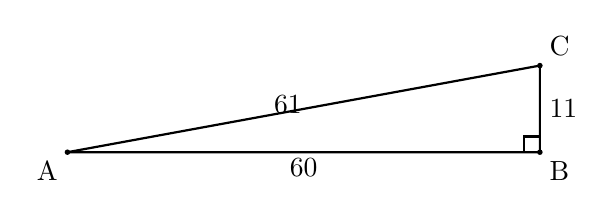
\begin{tikzpicture}
        % Define the coordinates of the triangle
        \coordinate (A) at (0,0);
        \coordinate (B) at (6,0);
        \coordinate (C) at (6,1.1);
        
        % Draw the triangle
        \draw[thick] (A) -- (B) -- (C) -- cycle;
        
        % Mark the right angle
        \draw[thick] (B) -- ++(-0.2,0) -- ++(0,0.2) -- ++(0.2,0);
        
        % Label the sides
        \node at (3,-0.2) {60};
        \node at (6.3,0.55) {11};
        \node at (2.8,0.6) {61};
        
        % Label the points
        \node[below left] at (A) {A};
        \node[below right] at (B) {B};
        \node[above right] at (C) {C};
        
        % Mark the points
        \fill (A) circle (1pt);
        \fill (B) circle (1pt);
        \fill (C) circle (1pt);
    \end{tikzpicture}
    \caption{Right triangle with labeled sides and vertices}
\end{figure}

\bigskip

Choose the correct answer for Figure 1:

\[
\begin{aligned}
    \text{A) } & \quad \sin A = \frac{61}{11} \\
    \text{B) } & \quad \sin A = \frac{60}{61} \\
    \text{C) } & \quad \sin A = \frac{11}{61} \\
    \text{D) } & \quad \sin A = \frac{11}{60}
\end{aligned}
\]

\bigskip



\footnote{Source: Math10, \emph{Trigonometry Problems}, \url{https://www.math10.com/problems/trigonometry-problems/easy/}}

\end{document}
